\chapter{System-Level Radiation Tests and Results}
\label{chapter:rad-tests-results}

This chapter presents and analyzes the system-level irradiation tests conducted at the CHARM and CC60 facilities. Tests that did not yield significant observations are documented in the appendices. The radiation characterization of the magnetic encoder, having been covered separately, is not repeated here.

All tests use the same demonstration position control implemented in firmware, in which a Timer/Counter commands a successive rotation of 90\textdegree{} at fixed time intervals, as described in Chapter~\ref{subsection:test-facilities-requirements}. The test bench is the same across all facilities, as described in the previous chapter.

\section{Pre-Irradiation System Performance}

\section{CHARM Test of the Initial Prototype}

This test took place at the CHARM facility in the overhead position. For this, the DUT was mounted on the conveyor as demonstrated in the following pictures.

This test proves very useful because it we have the chance to evaluate the system to SEE. The most sensitive component to SEE is the MCU and thus it is very useful to document the errors and calculate the cross-section between this and other tests. The system failed due to the gate drivers, and this failure was also verified in a cobalt test as will be presented in section \ref{sec:cc60-l6498d}.

\section{$^{60}$Co Irradiation Test of the Revised System}
\label{sec:cc60-l6498d}

The irradiation test was carried out at the CC60 facility using a Cobalt-60 source. For the purposes of the test, the motor setup was mounted on a frame in front of the radiation source, placed on a movable table at a specific distance that calibrates the dose rate. As shown in Figure~\ref{fig:cc60-revised}, the PCB was irradiated from the bottom side of the setup. This orientation was selected so that the aluminium structure and the motor would not shield part of the board from the incoming $\gamma$-radiation.

% \begin{figure}[H]
%   \centering
%   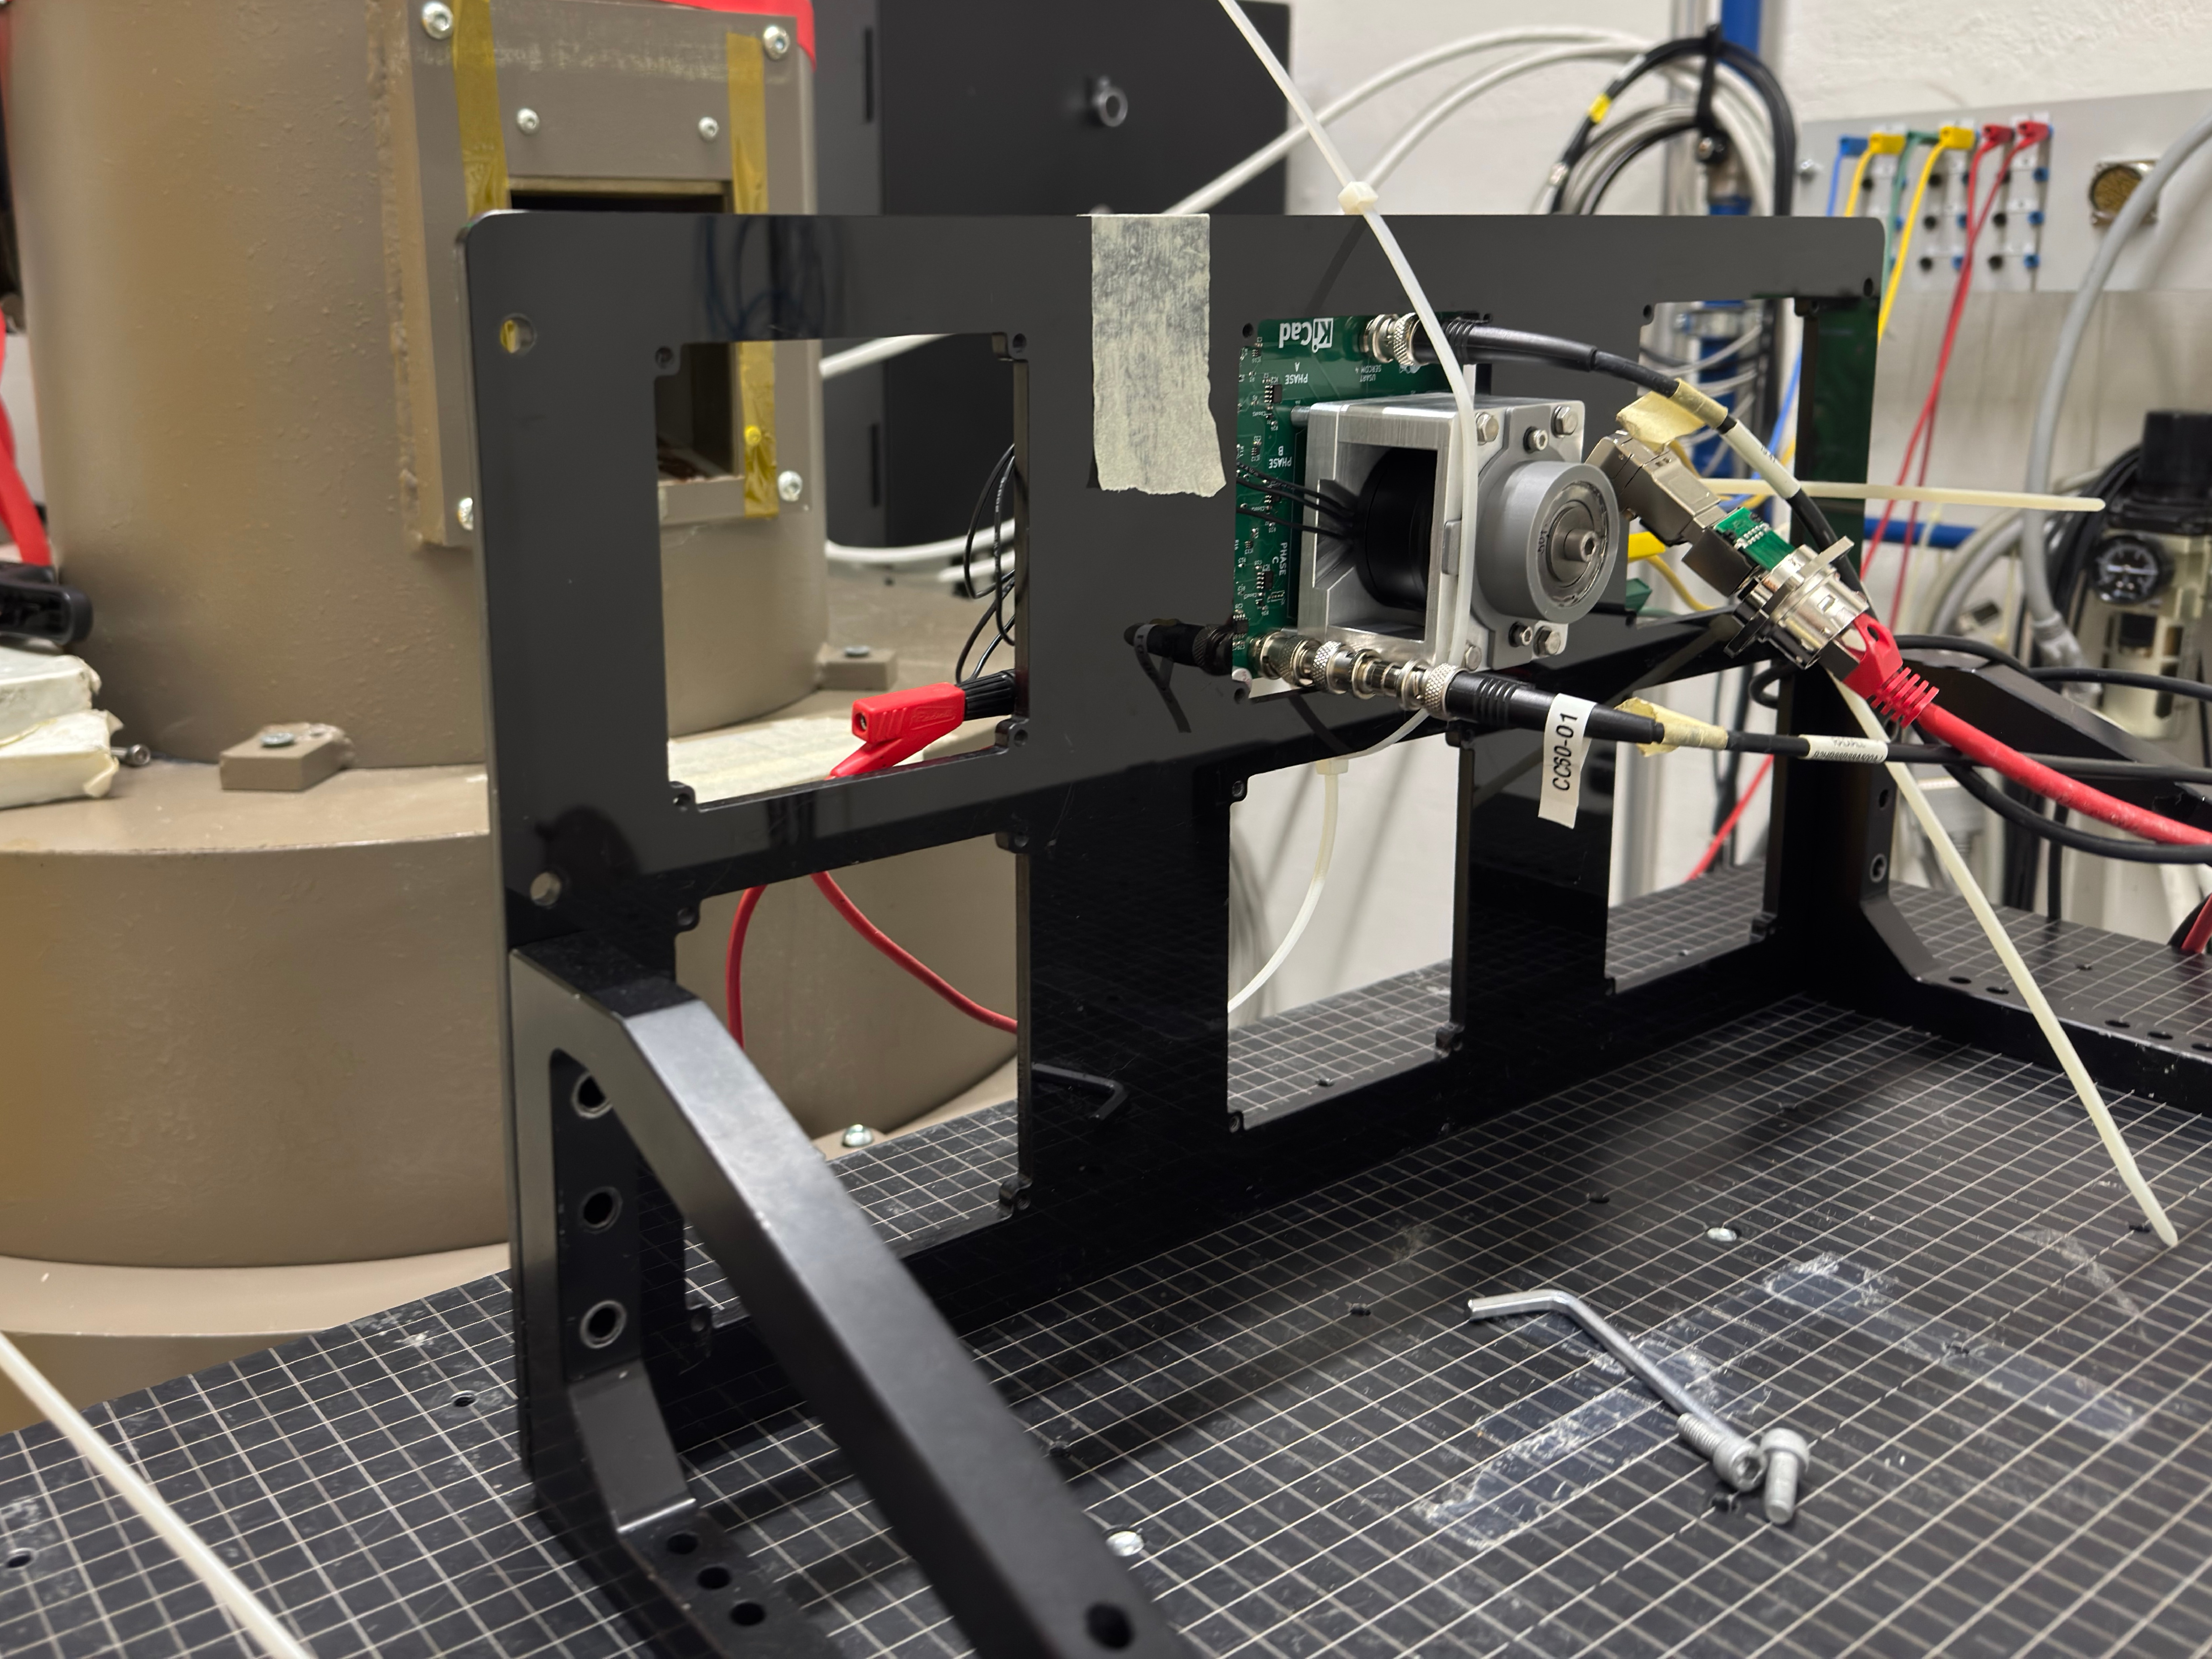
\includegraphics[width=0.8\textwidth,keepaspectratio]{06_RadiationTestsResults/images/System-Revised-CC60.JPG}
%   \caption{Image from the test setup before irradiation at CC60 facility}
%   \label{fig:cc60-revised}
% \end{figure}

For this test the dose rate was calibrated at 30 Gy/h. The system showed an unexpectedly quick degradation that lead it to permanent failure at a much lower TID than the initial target of 500 Gy.

The new testing procedures with the split voltage rails helped a lot to visualize how the components behaved during this test.

The test was driven to premature failure and failed to meet the target of 500 Gy. The point of failure is found at that many gray.




\section{$^{60}$Co Irradiation Test with NCP5183 Gate Drivers}

This test was performed two days after the previously described irradiation test and followed an almost identical procedure. The main difference was the replacement of the gate drivers with NCP5183 devices. After this modification, the setup remained fully functional up to an accumulated dose of 650 Gy. This value exceeded the initial expectations based on the estimated MCU tolerance and satisfied the initial target dose of 500 Gy.

An important objective of this test was to identify the accumulated dose at which the system began to lose controllability. For this purpose, the change in average current consumption was evaluated using a moving average over a 30 Gy dose window.

\subsection{Effects of TID on Components}

The effects of TID on the system components are evaluated in terms of current consumption, as shown in Figure~\ref{fig:cc60-ncp-currents}.

\begin{figure}[H]
  \centering
  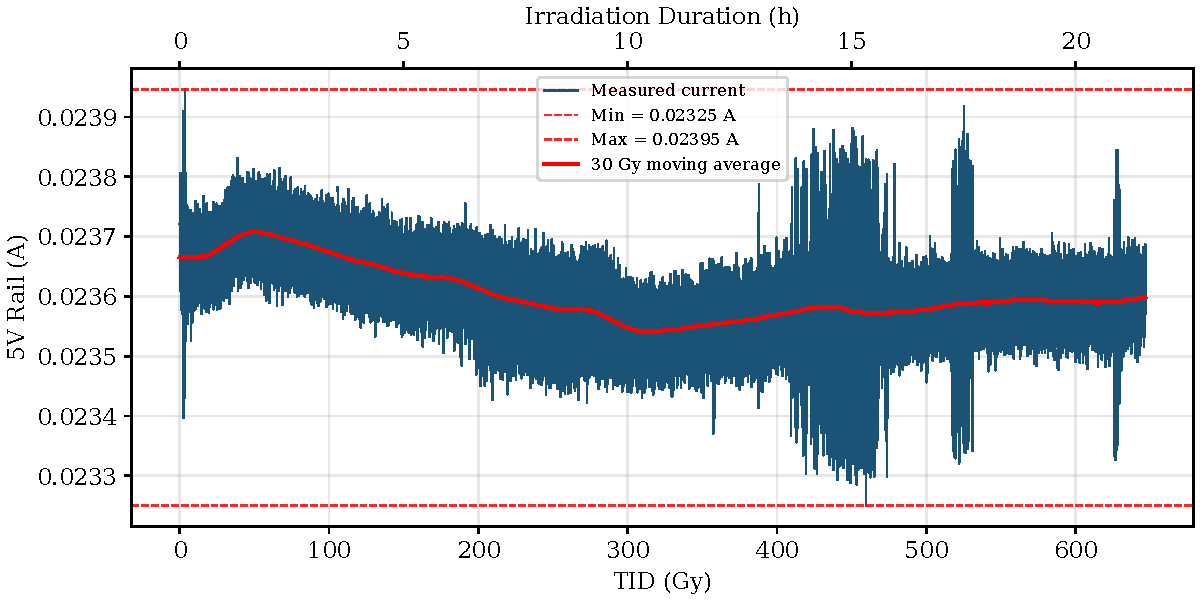
\includegraphics[width=0.82\textwidth,keepaspectratio]{06_RadiationTestsResults/cc60-ncp5183/Current_5V_Rail.pdf}
  \caption{Current consumption of the 5 V digital-logic rail during TID irradiation.}
  \label{fig:cc60-ncp-current-5v}
\end{figure}

\begin{figure}[H]
  \centering
  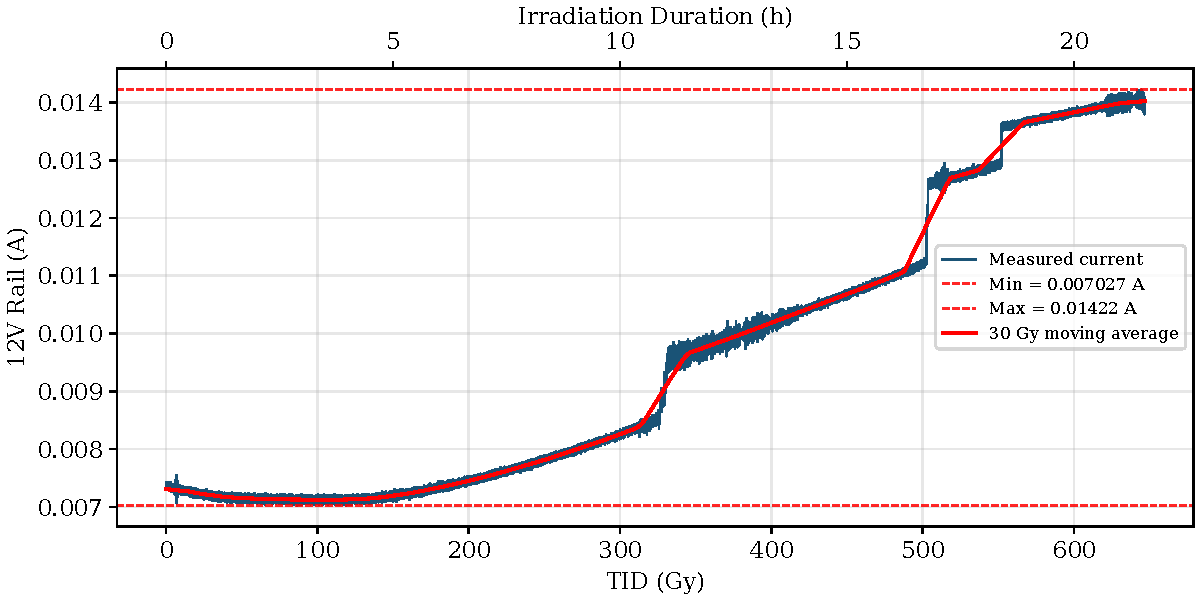
\includegraphics[width=0.82\textwidth,keepaspectratio]{06_RadiationTestsResults/cc60-ncp5183/Current_12V_Rail.pdf}
  \caption{Current consumption of the 12 V gate-driver and voltage-reference rail during TID irradiation.}
  \label{fig:cc60-ncp-current-12v}
\end{figure}

\begin{figure}[H]
  \centering
  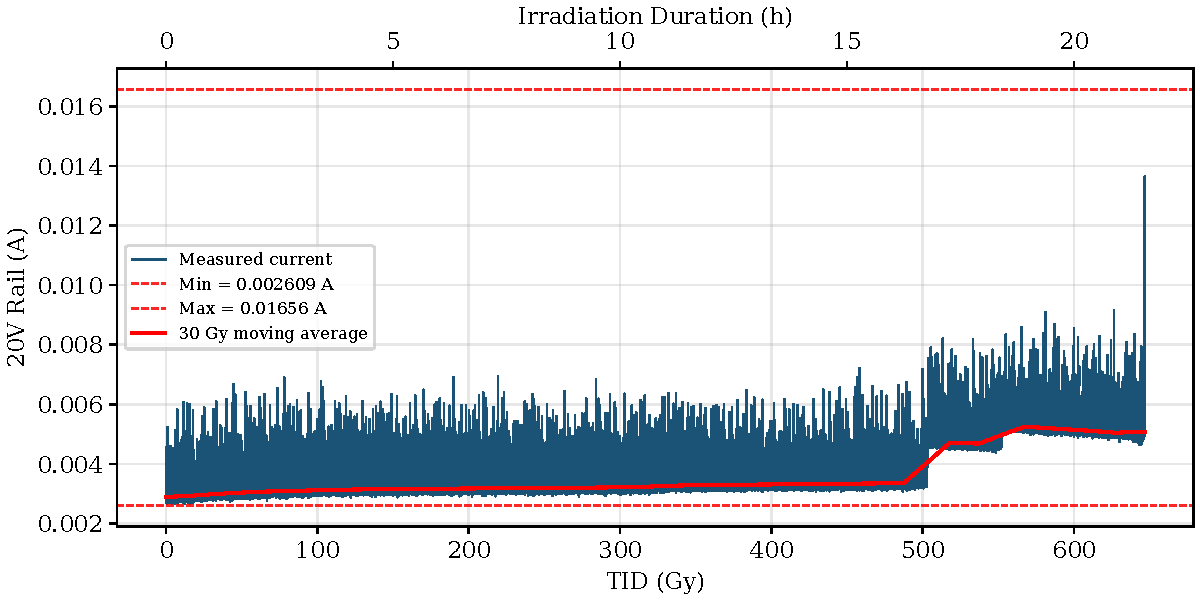
\includegraphics[width=0.82\textwidth,keepaspectratio]{06_RadiationTestsResults/cc60-ncp5183/Current_20V_Rail.pdf}
  \caption{Current consumption of the 20 V motor-phase rail during TID irradiation.}
  \label{fig:cc60-ncp-current-20v}
\end{figure}

The current consumption of the 5 V rail remained very stable throughout the irradiation test. In contrast, the 12 V rail, which supplies the voltage reference and gate drivers, exhibited a significant increase after an accumulated dose of approximately 300 Gy. Additional discrete increases were observed at approximately 500 Gy and 550 Gy.

The current consumption of the 20 V motor supply remained well regulated during the irradiation run. However, discrete increases were observed during the same dose intervals as those seen on the 12 V rail, suggesting a possible correlation between the two effects. Since the motor was tested without mechanical load and the measured currents remained very low, no firm conclusion can be drawn regarding the behaviour of the system under higher-load operating conditions.

A summary of the degradation in current consumption is provided in Table~\ref{tab:cc60-ncp-current-statistics}.

\begin{table}[H]
  \centering
  \begin{tabular}{lccccc}
        \toprule
        Rail & Minimum (A) & Maximum (A) & Starting (A) & Final (A) & Change (\%) \\
        \midrule
        5 V & 0.0233 & 0.0239 & 0.0237 & 0.0236 & -0.42 \\
        12 V & 0.0070 & 0.0142 & 0.0074 & 0.0140 & 89.15 \\
        20 V & 0.0026 & 0.0166 & 0.0029 & 0.0070 & 144.50 \\
        \bottomrule
    \end{tabular}
    \caption{Current consumption statistics of the three voltage rails during irradiation.}
    \label{tab:cc60-ncp-current-statistics}
\end{table}

\subsection{Repeatability Degradation Analysis over Time}

Following the methodology described in subsection~\ref{subsection:model-accuracy-repeatability}, the repeatability of the measured rotor position was evaluated over the full irradiation cycle. The results are shown in Figure~\ref{fig:cc60-ncp-repeatability-local}.

\begin{figure}[H]
  \centering

  \begin{minipage}{0.48\textwidth}
    \centering
    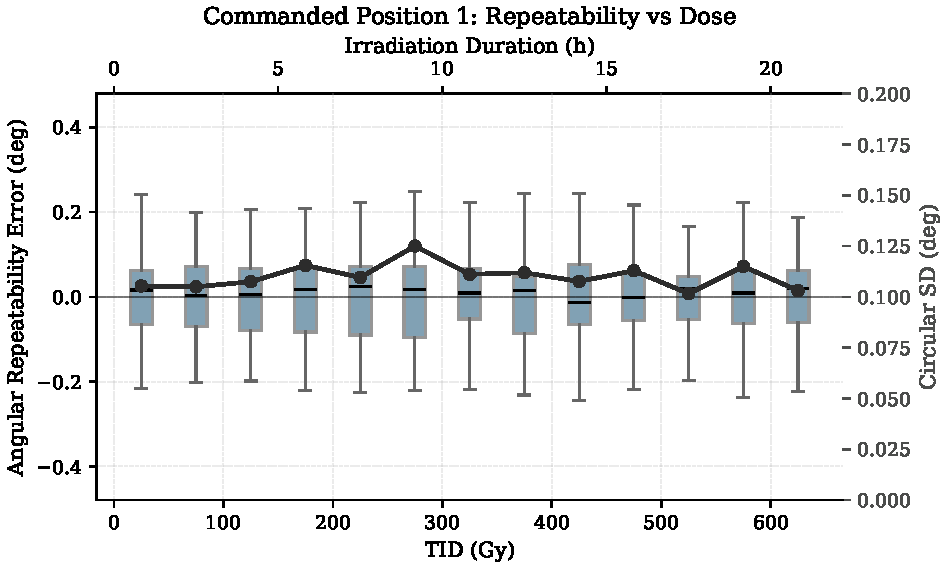
\includegraphics[width=\textwidth,keepaspectratio]{06_RadiationTestsResults/cc60-ncp5183/_Repeatability_Boxplot_Angle_1_Local.pdf}
  \end{minipage}
  \hfill
  \begin{minipage}{0.48\textwidth}
    \centering
    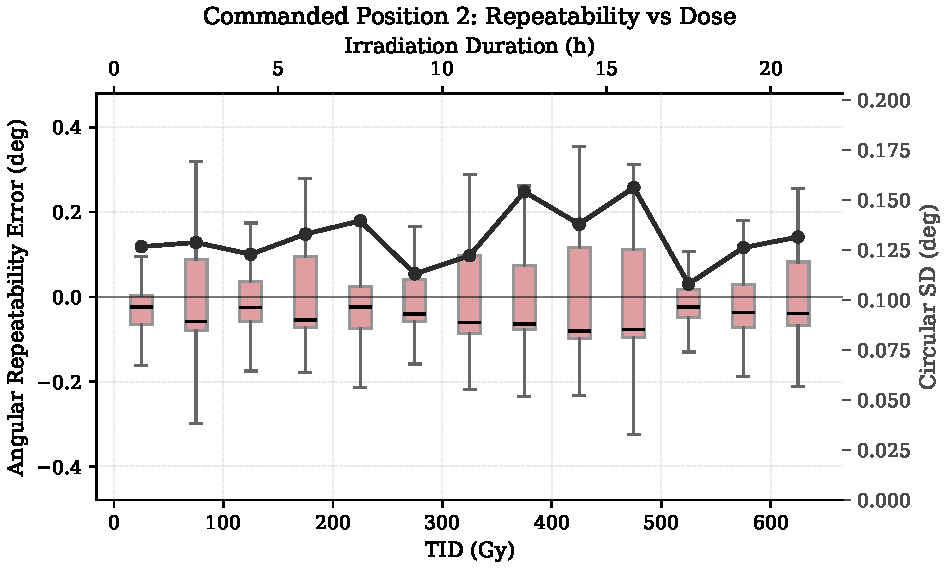
\includegraphics[width=\textwidth,keepaspectratio]{06_RadiationTestsResults/cc60-ncp5183/_Repeatability_Boxplot_Angle_2_Local.pdf}
  \end{minipage}

  \vspace{0.3cm}

  \begin{minipage}{0.48\textwidth}
    \centering
    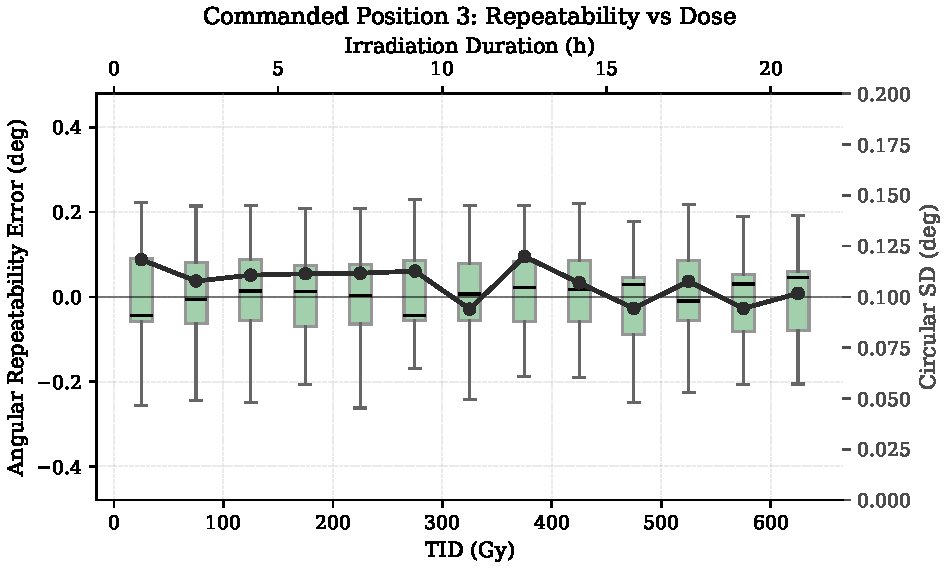
\includegraphics[width=\textwidth,keepaspectratio]{06_RadiationTestsResults/cc60-ncp5183/_Repeatability_Boxplot_Angle_3_Local.pdf}
  \end{minipage}
  \hfill
  \begin{minipage}{0.48\textwidth}
    \centering
    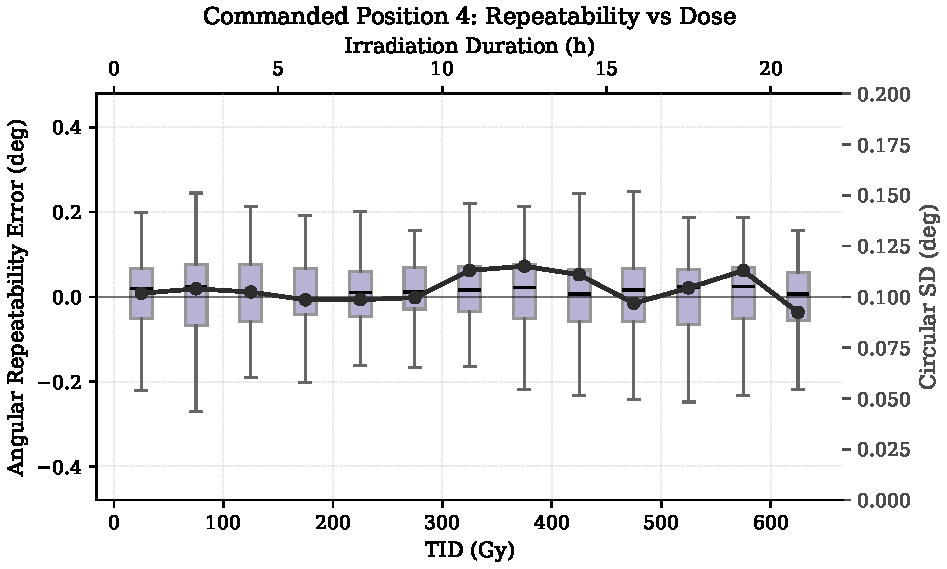
\includegraphics[width=\textwidth,keepaspectratio]{06_RadiationTestsResults/cc60-ncp5183/_Repeatability_Boxplot_Angle_4_Local.pdf}
  \end{minipage}

  \caption{Repeatability analysis of the measured rotor position during irradiation for angles 1--4.}
  \label{fig:cc60-ncp-repeatability-local}
\end{figure}

\begin{figure}[H]
  \centering
  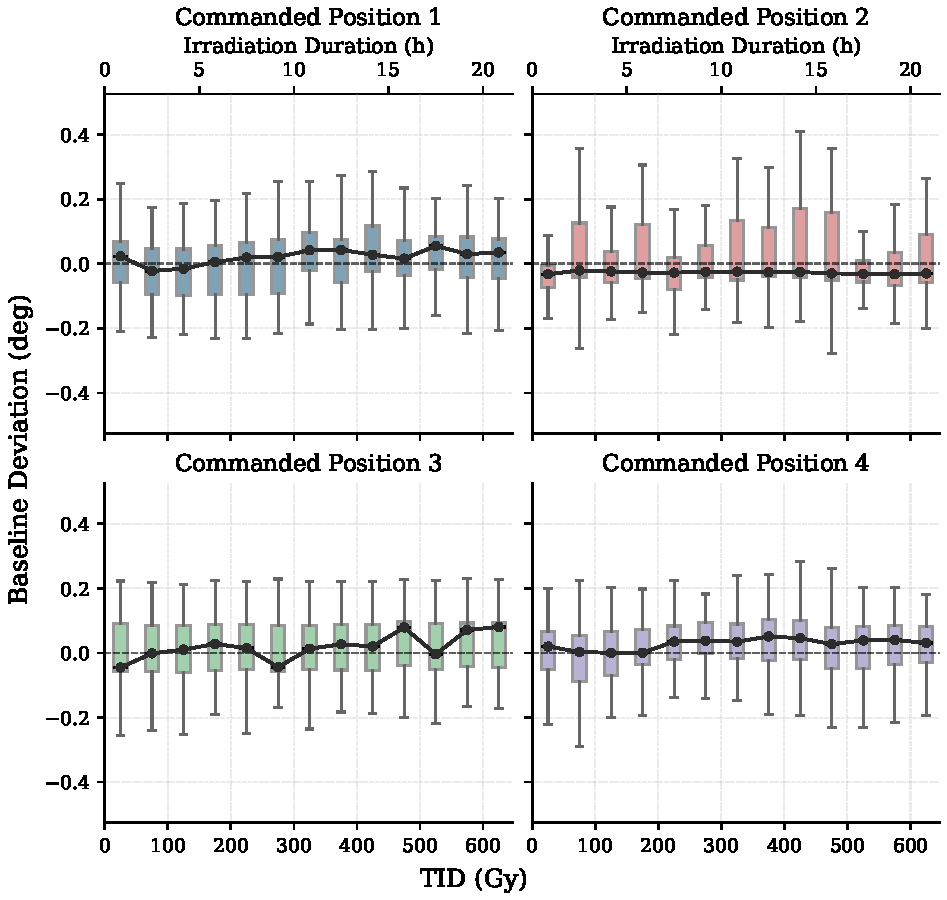
\includegraphics[width=\textwidth,keepaspectratio]{06_RadiationTestsResults/cc60-ncp5183/_Repeatability_Boxplot_Combined_Global.pdf}
  \caption{Evolution of the TC4 interrupt period during irradiation. The trendline highlights the gradual decrease in the interrupt period as the accumulated dose increases.}
\end{figure}

\begin{figure}[H]
  \centering

  \begin{minipage}{0.48\textwidth}
    \centering
    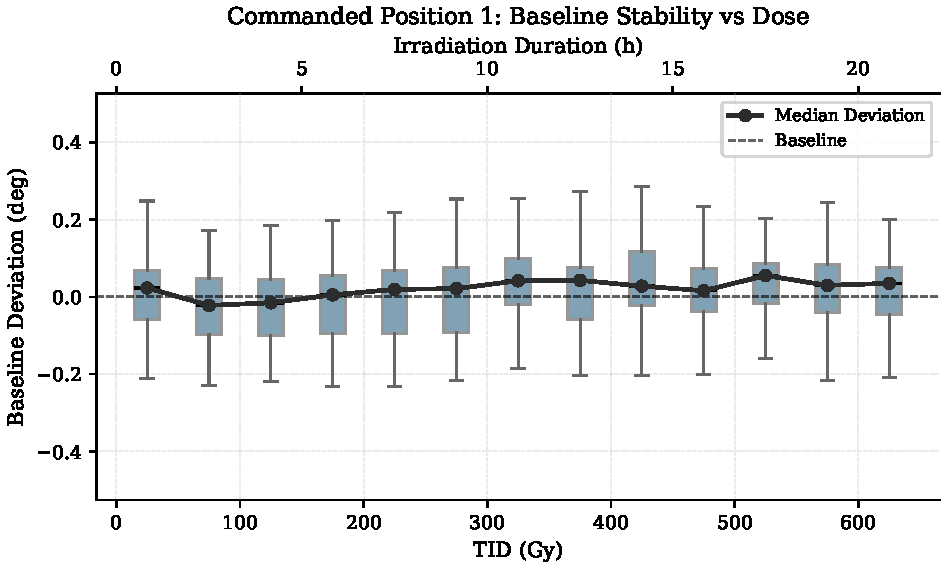
\includegraphics[width=\textwidth,keepaspectratio]{06_RadiationTestsResults/cc60-ncp5183/_Repeatability_Boxplot_Angle_1_Global.pdf}
  \end{minipage}
  \hfill
  \begin{minipage}{0.48\textwidth}
    \centering
    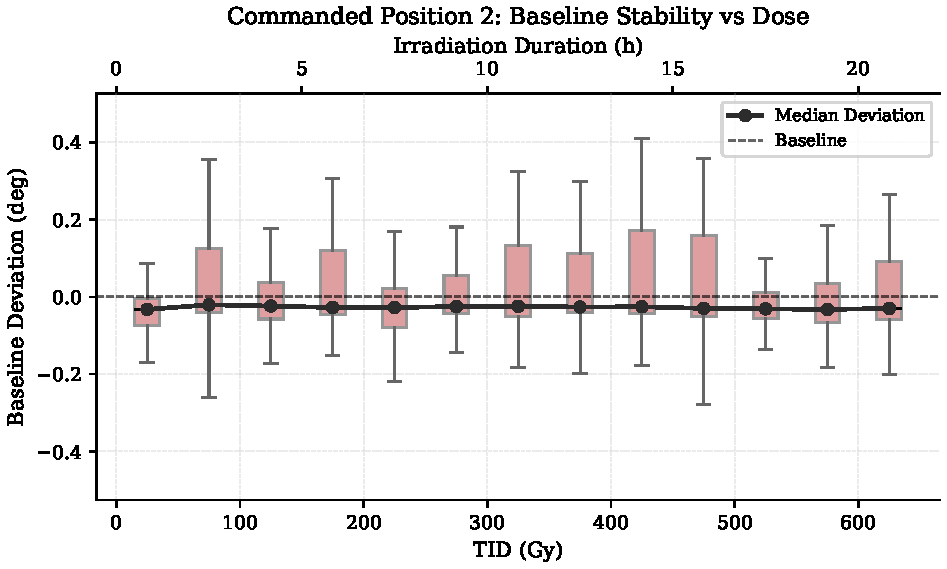
\includegraphics[width=\textwidth,keepaspectratio]{06_RadiationTestsResults/cc60-ncp5183/_Repeatability_Boxplot_Angle_2_Global.pdf}
  \end{minipage}

  \vspace{0.3cm}

  \begin{minipage}{0.48\textwidth}
    \centering
    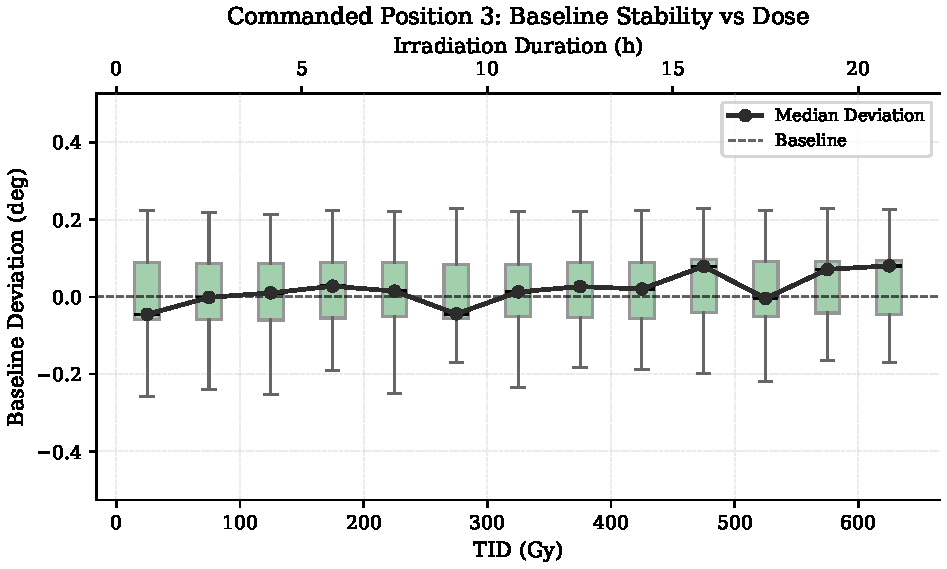
\includegraphics[width=\textwidth,keepaspectratio]{06_RadiationTestsResults/cc60-ncp5183/_Repeatability_Boxplot_Angle_3_Global.pdf}
  \end{minipage}
  \hfill
  \begin{minipage}{0.48\textwidth}
    \centering
    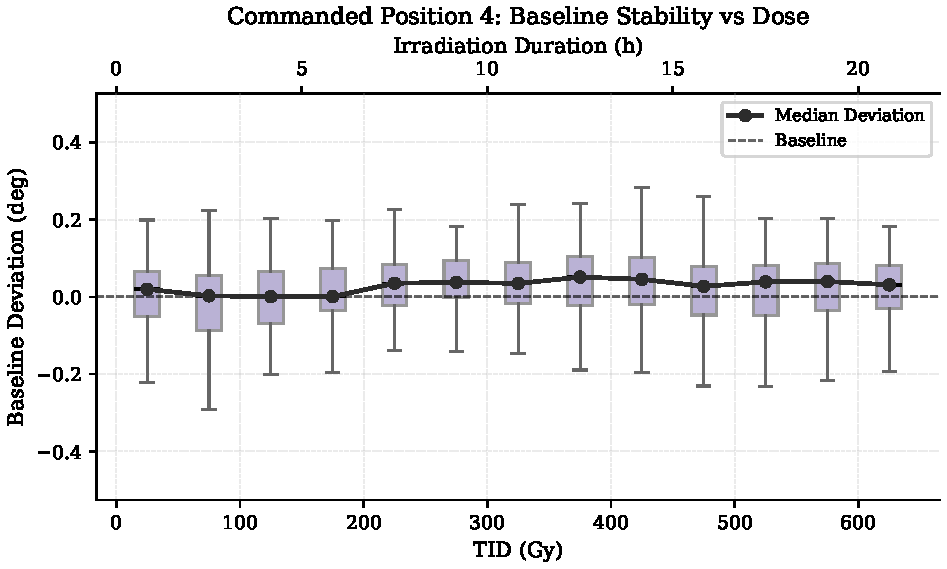
\includegraphics[width=\textwidth,keepaspectratio]{06_RadiationTestsResults/cc60-ncp5183/_Repeatability_Boxplot_Angle_4_Global.pdf}
  \end{minipage}

  \caption{Repeatability analysis of the measured rotor position during irradiation for angles 1--4.}
  \label{fig:cc60-ncp-repeatability-global}
\end{figure}

\begin{figure}[H]
  \centering

  \begin{minipage}{0.48\textwidth}
    \centering
    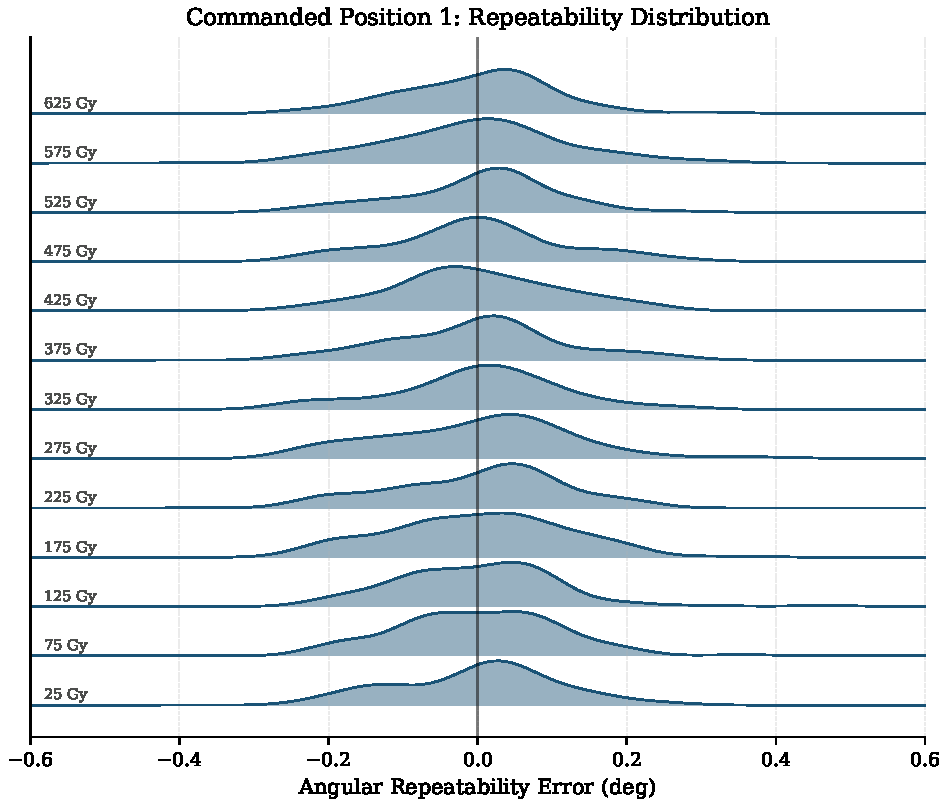
\includegraphics[width=\textwidth,keepaspectratio]{06_RadiationTestsResults/cc60-ncp5183/_Repeatability_Ridgeline_Angle_1_Local.pdf}
  \end{minipage}
  \hfill
  \begin{minipage}{0.48\textwidth}
    \centering
    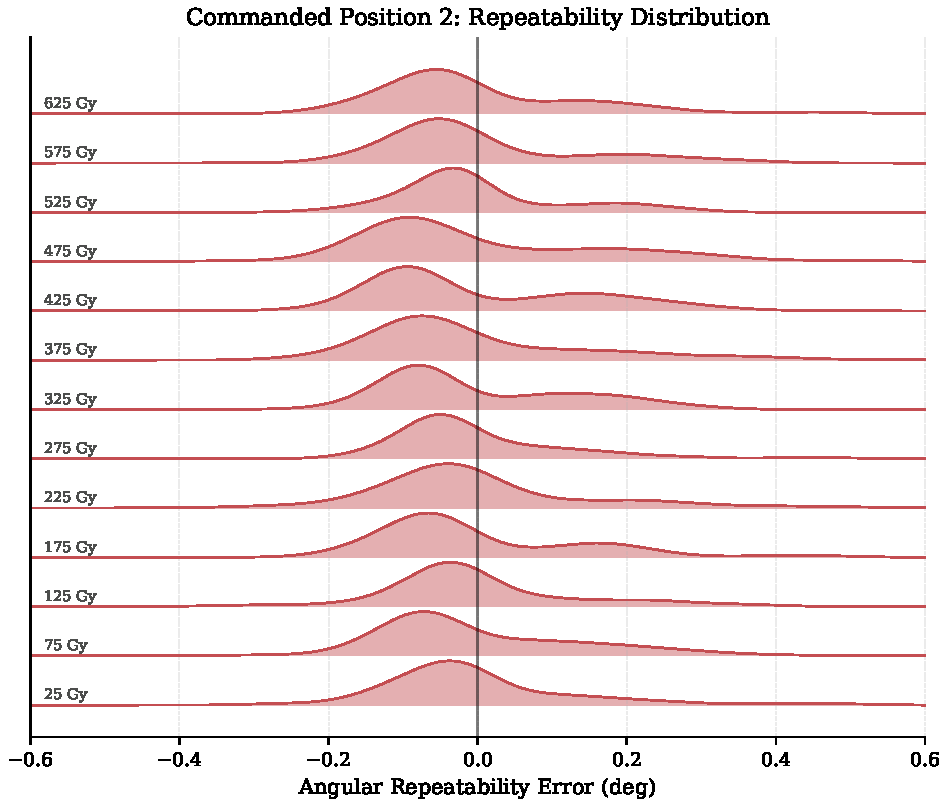
\includegraphics[width=\textwidth,keepaspectratio]{06_RadiationTestsResults/cc60-ncp5183/_Repeatability_Ridgeline_Angle_2_Local.pdf}
  \end{minipage}

  \vspace{0.3cm}

  \begin{minipage}{0.48\textwidth}
    \centering
    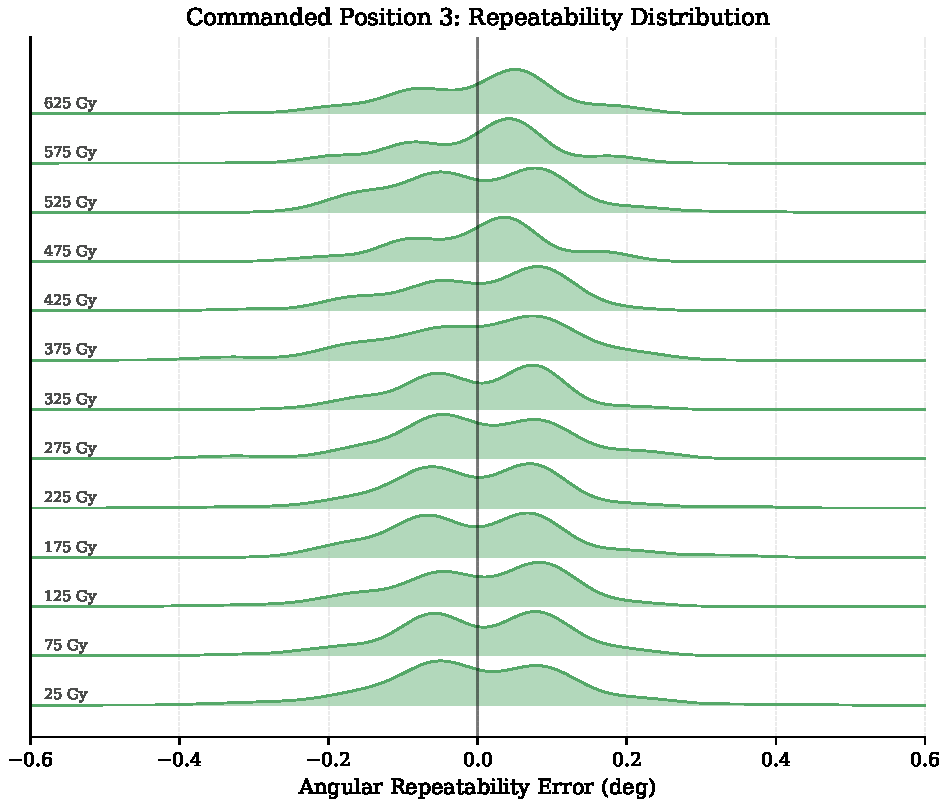
\includegraphics[width=\textwidth,keepaspectratio]{06_RadiationTestsResults/cc60-ncp5183/_Repeatability_Ridgeline_Angle_3_Local.pdf}
  \end{minipage}
  \hfill
  \begin{minipage}{0.48\textwidth}
    \centering
    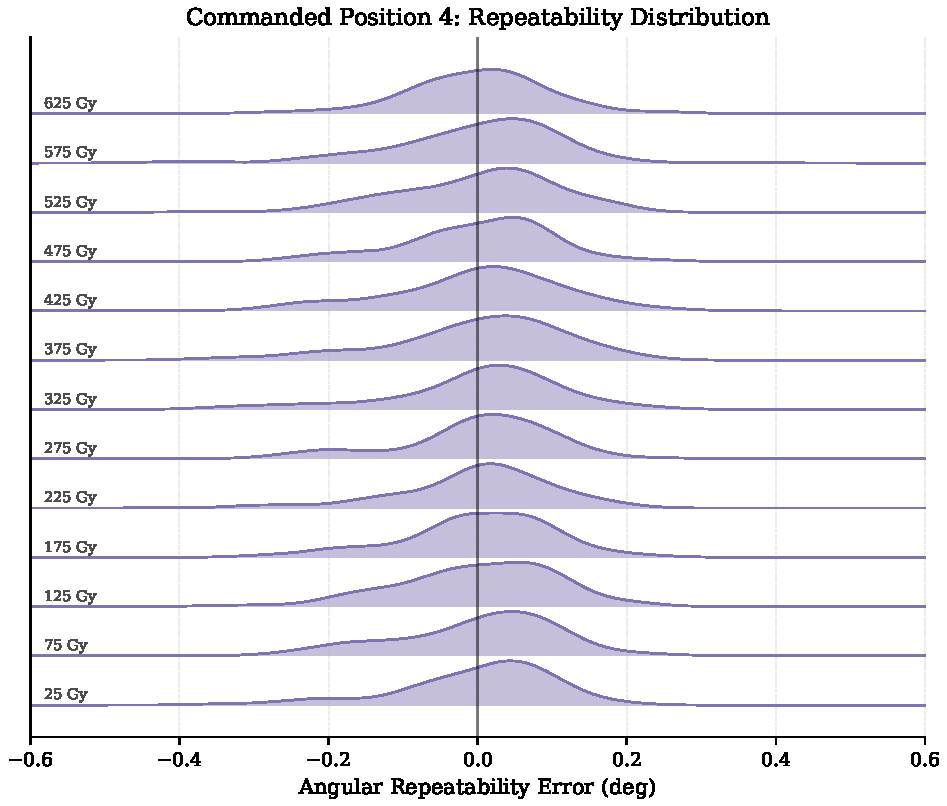
\includegraphics[width=\textwidth,keepaspectratio]{06_RadiationTestsResults/cc60-ncp5183/_Repeatability_Ridgeline_Angle_4_Local.pdf}
  \end{minipage}

  \caption{Repeatability analysis of the measured rotor position during irradiation for angles 1--4 using local coordinates.}
  \label{fig:cc60-ncp-repeatability-ridgeline-local}
\end{figure}

\begin{figure}[H]
  \centering

  \begin{minipage}{0.48\textwidth}
    \centering
    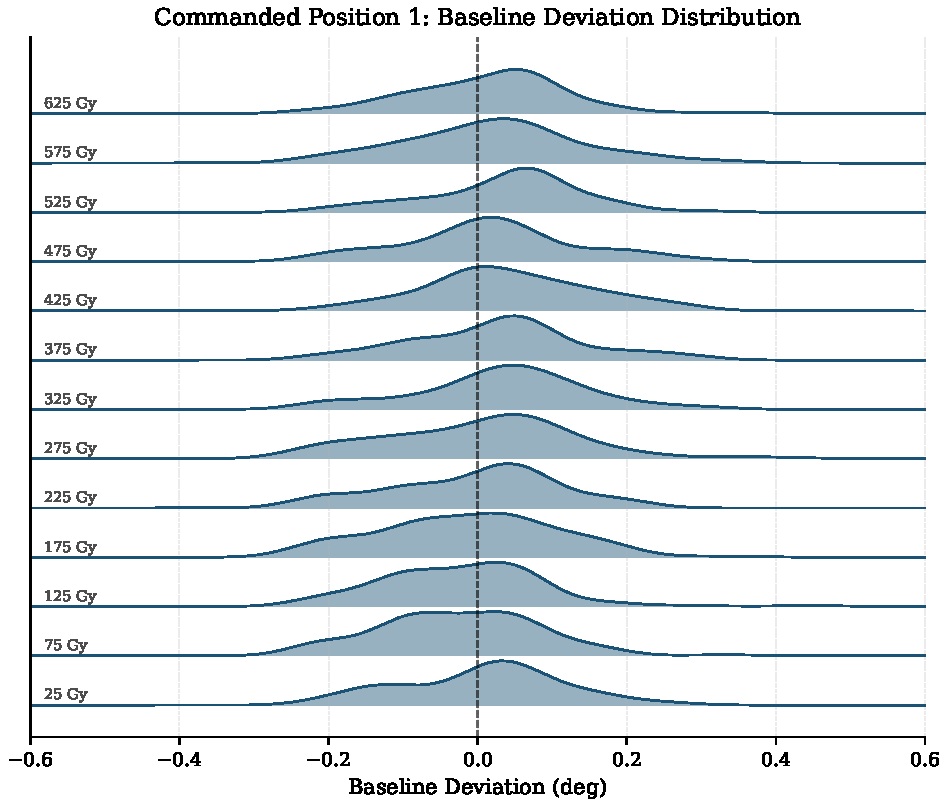
\includegraphics[width=\textwidth,keepaspectratio]{06_RadiationTestsResults/cc60-ncp5183/_Repeatability_Ridgeline_Angle_1_Global.pdf}
  \end{minipage}
  \hfill
  \begin{minipage}{0.48\textwidth}
    \centering
    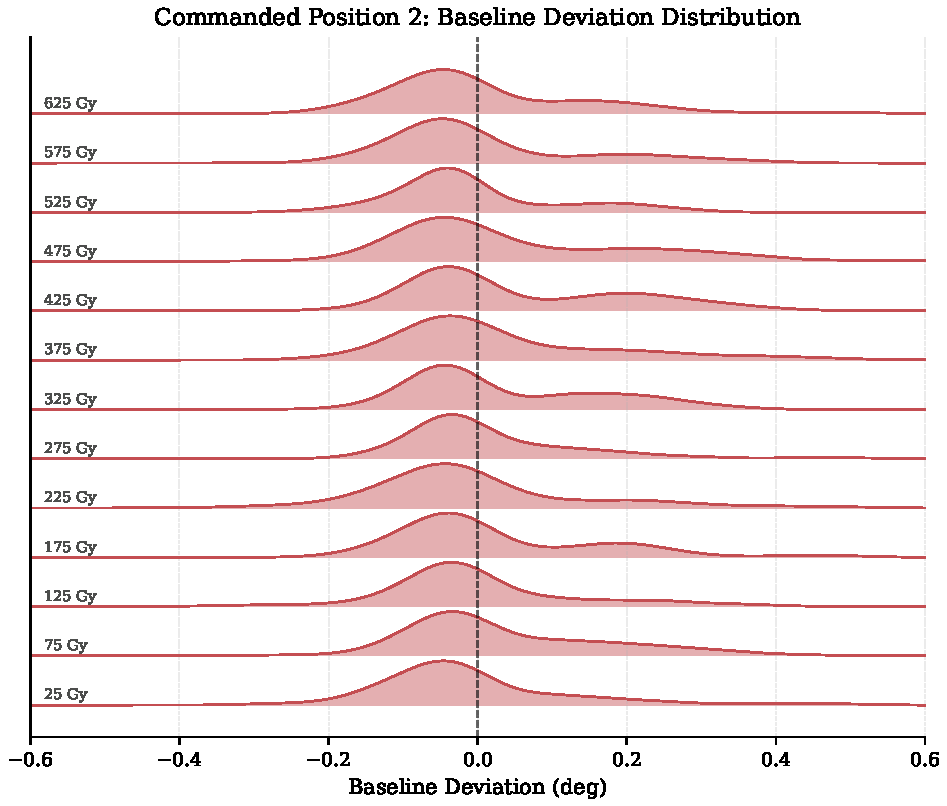
\includegraphics[width=\textwidth,keepaspectratio]{06_RadiationTestsResults/cc60-ncp5183/_Repeatability_Ridgeline_Angle_2_Global.pdf}
  \end{minipage}

  \vspace{0.3cm}

  \begin{minipage}{0.48\textwidth}
    \centering
    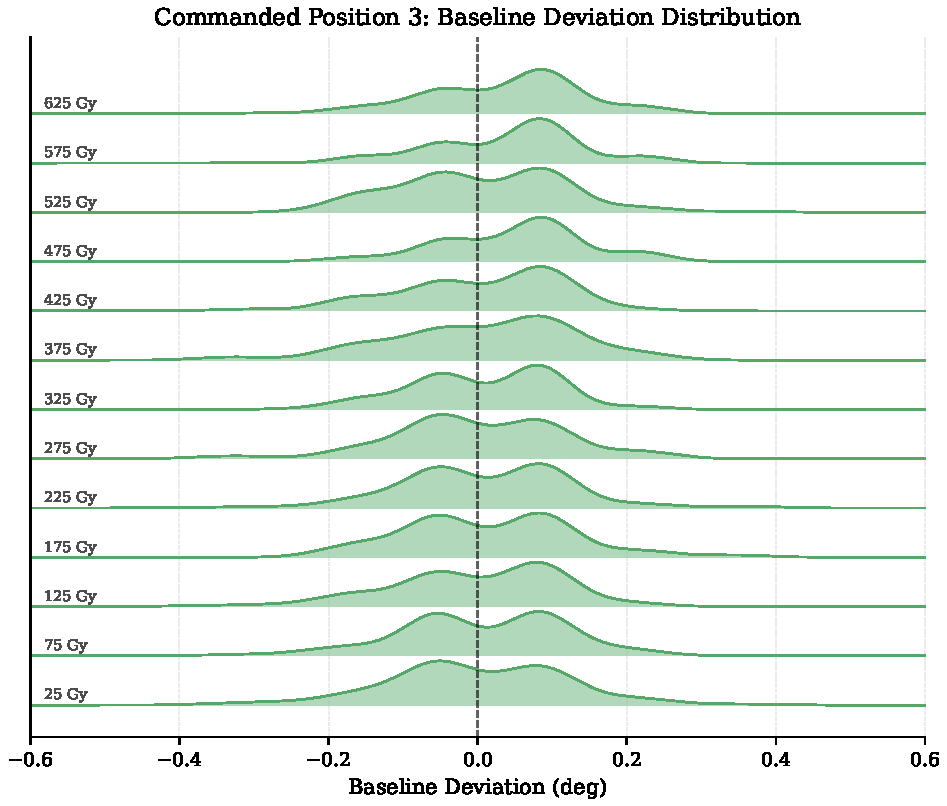
\includegraphics[width=\textwidth,keepaspectratio]{06_RadiationTestsResults/cc60-ncp5183/_Repeatability_Ridgeline_Angle_3_Global.pdf}
  \end{minipage}
  \hfill
  \begin{minipage}{0.48\textwidth}
    \centering
    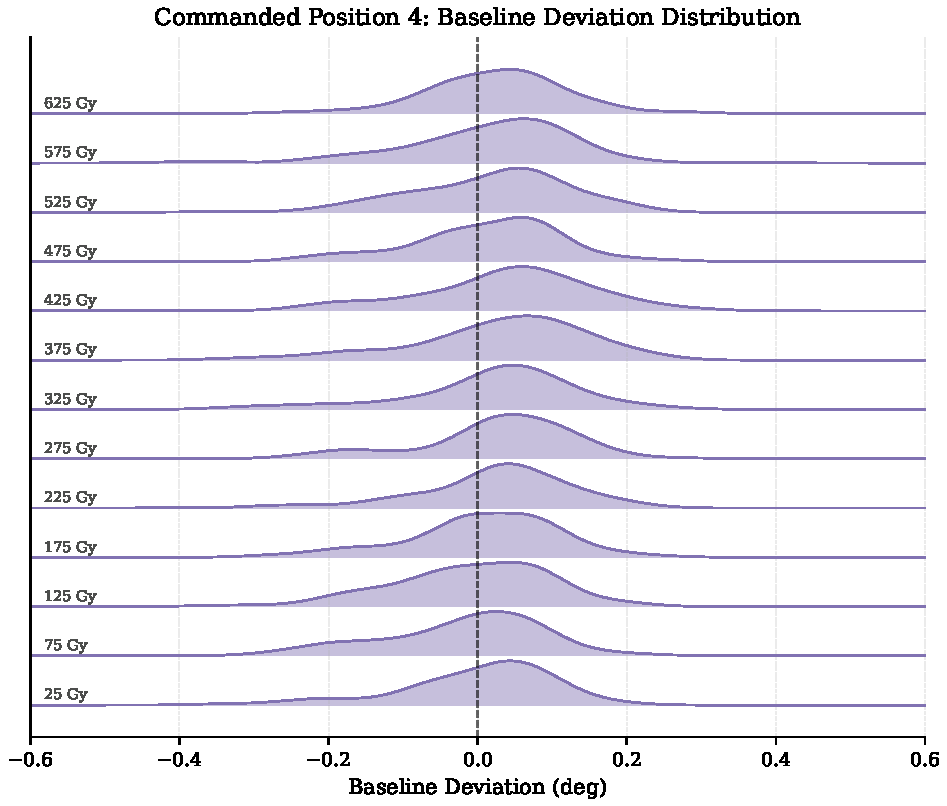
\includegraphics[width=\textwidth,keepaspectratio]{06_RadiationTestsResults/cc60-ncp5183/_Repeatability_Ridgeline_Angle_4_Global.pdf}
  \end{minipage}

  \caption{Repeatability analysis of the measured rotor position during irradiation for angles 1--4 using global coordinates.}
  \label{fig:cc60-ncp-repeatability-ridgeline-global}
\end{figure}



The position control performance of the system was evaluated across the full irradiation window from 0 to \SI{647}{\gray} through two complementary repeatability metrics.

The first metric is the \textbf{local repeatability} that is defined as the cycle to cycle scatter of the settled resolver angles about the per-dose mean. That means that each \SI{50}{\gray} interval is treated independently for the settled angles. The circular standard deviation stayed withing \SIrange{0.10}{0.13}{\degree} for all four commanded angles and showed no significant trend with the accumulated dose.

The second metric is the \textbf{global repeatability} which refers to the deviation between the settled angles across the whole irradiation period and the settled angle of the irradiation baseline of derived from the first \SI{60}{\gray} of data. The per-bin median drift remained within \SI{\pm 0.05}{\degree} across the full dose range, well within the intrinsic sensor noise floor and an order of magnitude below the AS5047P integral non-linearity of \SI{\pm 0.8}{\degree}. Thus, the conclusion is that there is no observed systematic drift but only control inaccuracies.

These results are confirmed by three independent representations of the same data. The boxplots show constant box height (scatter) and median positions that remain on the zero reference throughout the irradiation. The ridgeline distributions show that the shape, width and center of the repeatability error distribution are preserved from \SI{25}{\gray} to \SI{625}{\gray}, with no progressive shift or broadening observable with increasing dose.

The observed mild asymmetry of the repeatability distribution — with the peak sitting slightly positive relative to zero — is consistent across all dose levels and all angle states. It reflects a structural property of the motor settle dynamics (approach-direction asymmetry and cogging) rather than any radiation-induced effect, and is present from the first measurement bin at \SI{25}{\gray}. This indicates that, although the current consumption of the system increased during irradiation, the short-term repeatability of the rotor position measurement remained stable.

\subsection{Accuracy Degradation Analysis over Time}

\subsection{Degradation of Timer/Counter Accuracy over Time}

During the degradation analysis, an additional timing-related effect was observed. When several motion periods were overlaid on the same time frame, the corresponding waveforms did not remain perfectly aligned. Instead, they gradually shifted apart as the irradiation dose increased. This indicated that the timing of the periodic interrupt responsible for updating the rotor position was not constant during the test.

For this reason, the period of the TC4 interrupt was analyzed over the full irradiation cycle. The resulting trend is shown in Figure~\ref{fig:cc60-ncp-tc4}. The analysis shows that the interrupt period gradually decreased with accumulated dose, meaning that the interrupt was triggered slightly faster towards the end of the irradiation test.

\begin{figure}[H]
  \centering
  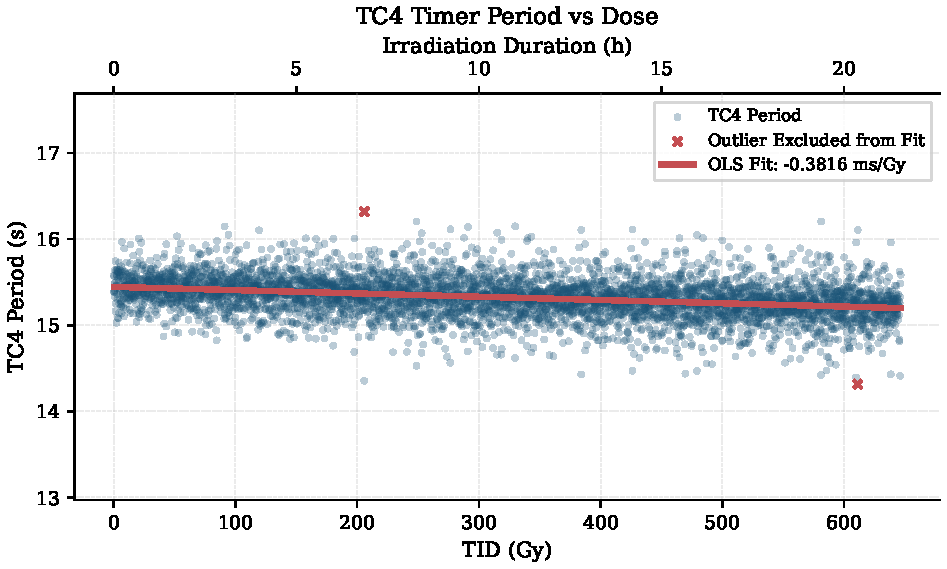
\includegraphics[width=\textwidth,keepaspectratio]{06_RadiationTestsResults/cc60-ncp5183/_TC4_Timer_Period_Stability_vs_TID.pdf}
  \caption{Evolution of the TC4 interrupt period during irradiation. The trendline highlights the gradual decrease in the interrupt period as the accumulated dose increases.}
  \label{fig:cc60-ncp-tc4}
\end{figure}

The numerical change in the TC4 interrupt period is summarized in Table~\ref{tab:cc60-ncp-tc4-period-summary}. The fitted trend corresponds to a total decrease of approximately 246.8~ms over the irradiation cycle, equal to a relative decrease of approximately 1.6\%.

\begin{table}[H]
\centering
\begin{tabular}{lcccc}
    \toprule
    & Initial Duration (s) & Final Duration (s) & Decrease (ms) & Decrease (\%) \\
    \midrule
    TC4 IRQ Period & 15.4460 & 15.1992 & 246.8 & 1.598 \\
    \bottomrule
\end{tabular}
    \caption{Summary of the TC4 interrupt period drift during irradiation.}
\label{tab:cc60-ncp-tc4-period-summary}
\end{table}

Based on the firmware clock configuration, the TC4/TC5 peripheral clock is supplied by generic clock generator~2. This generator is configured from the DFLL48M clock source with a division factor of six, resulting in an expected TC4 generic clock of approximately 8~MHz. Therefore, the TC4 interrupt period is directly dependent on the DFLL48M-derived clock path.

The interrupt itself is not generated directly by the 48~MHz clock. Instead, TC4 counts timer ticks derived from this clock. After division by the generic clock generator and the TC4 prescaler, the timer counter reaches its configured overflow or compare-match condition. At that point, the corresponding interrupt flag is set and the interrupt request is forwarded to the NVIC. Consequently, if the DFLL48M-derived clock becomes slightly faster, TC4 reaches the interrupt condition sooner and the measured interrupt period becomes shorter.

This means that the observed period reduction is most likely related to drift in the DFLL48M-derived timer clock path, rather than to the 32.768~kHz oscillator directly. Although the internal 32.768~kHz oscillator is enabled in the clock configuration, it is assigned to generic clock generator~1 and is not the generator used by TC4. In addition, the DFLL is enabled without closed-loop correction in this configuration, meaning that its output frequency depends on the programmed coarse and fine calibration values. This makes the open-loop DFLL48M clock a plausible source of the measured timing drift.

The measured decrease of approximately 1.6\% in the interrupt period corresponds to an approximately 1.6\% increase in the effective timer clock frequency. In this test, the drift remained small and did not appear to compromise the operation of the system. However, since the firmware architecture is event-driven, excessive clock drift could eventually affect the timing of scheduled rotor-position updates and could lead to loss of synchronization or controllability. Future irradiation tests should therefore monitor the stability of the individual clock sources and derived clocks separately, especially the DFLL48M output, the generic clock supplied to TC4, and the low-frequency reference clocks.